
\noindent\textbf{4.} O problema \proc{2-sat} consiste na restrição de \proc{sat} a instâncias $X$ e $C$ em que toda cláusula de $C$ tem exatamente dois literais. Mostre que o \proc{2-sat} está em P, ou seja, descreva um algoritmo polinomial que resolva o \proc{2-sat}.\\[6pt]
\textcolor{red}{\textbf{Resposta:}} Podemos resolver esse 2-sat transformando esse problema em uma busca de caminho em grafos.

\textbf{Construção}: Seja $\Psi$ uma Forma Conjuntiva Normal com $n$ variáveis e $m$ clausulas. Vamos criar um grafo $G = (V, E)$ com $2n$ vértices, cada par de vértices representa uma variável de $\Psi$ onde um vértice representa a variável como literal e outro vértice a variável como o literal negado. Para cada clausula $(a \vee b)$, criaremos uma aresta direcionada de $\bar{a}$ para $b$ e de $\bar{b}$ para $a$. Essas arestas significam que se $a$ não é verdadeiro, então $b$ deve ser verdadeiro e vice-versa. Isso implica que existe uma aresta direcionada $(a,b)$ em $G$ se e somente se existe uma clausula $\bar{a} \vee b$ em $\Psi$.

Exemplo:

\[\Psi = (\bar{x} \vee y) \wedge (\bar{y} \vee x) \wedge (x \vee \bar{z}) \wedge (z \vee y) \]

\begin{figure}[H]  
  \centering  
 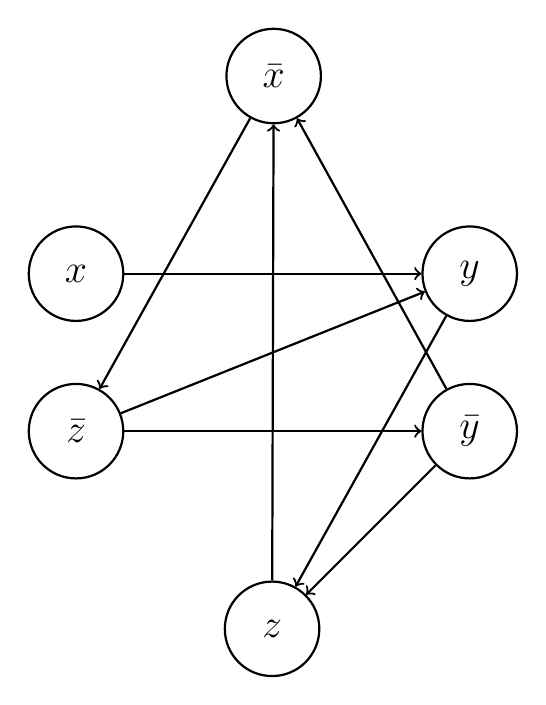
\begin{tikzpicture}[->, auto, node distance=5cm, thick, main_node/.style={circle,draw,font=\sffamily\Large\bfseries, minimum size=1.2cm, align=center}]
  
  \node[main_node] (1) [] {$\bar{x}$};
  \node[main_node] (2) [below left of=1, node distance=3.55cm] {$x$};
  \node[main_node] (3) [right of=2] {$y$};
  \node[main_node] (4) [below of=3, node distance=2cm] {$\bar{y}$};
  \node[main_node] (5) [below left of=4, node distance=3.55cm] {$z$};
  \node[main_node] (6) [left of=4] {$\bar{z}$};  
  
%   \node[main_node] (9) [below of=8, node distance=1.5cm] {G};  
	     
  \path[every node/.style={font=\sffamily\small}]
    (1)	edge node {} (6)
    (2) edge node {} (3)
    (3) edge node {} (5)
    (4) edge node {} (1)
	edge node {} (5)
    (5) edge node {} (1)    
    (6) edge node {} (3)
	edge node {} (4);
  \end{tikzpicture}
\end{figure}

\textbf{Corretude}:

\textbf{Afirmação}: Se $G$ Contém um caminho de $a$ a $b$, então ele também contém um caminho de $\bar{a}$ a $\bar{b}$.

\textbf{Prova}: seja um $p = a,a_1,a_2, .. a_k, b$ um caminho de $a$ a $b$. Por construção sabemos que se existe uma aresta  $(x,y)$ então também existe uma aresta $(\bar{x}, \bar{y})$, logo as arestas $(\bar{b}, \bar{a_k}), (\bar{a_k}, \bar{a_{k-1}}), .., (\bar{a_2}, \bar{a_1}), (\bar{a_1}, \bar{a})$ existem, portanto existe um caminho de $\bar{y}$ até $\bar{x}$.

\textbf{Afirmação}: uma 2-formula normal conjuntiva $\Psi$ não é satisfazivel se e somente se existe uma variável $x$ tal que:
\begin{itemize}
 \item Existe um caminho de $x$ a $\bar{x}$ no grafo gerado $G$.
 \item Existe um caminho de $\bar{x}$ a $x$ no grafo gerado $G$.
\end{itemize}

\textbf{Prova}: Vamos assumir por contradição que existem os caminho $p$ e $p'$ tal que $p$ vai de $x$ a $\bar{x}$ e $p'$ vai de $\bar{x}$ até $x$ para alguma variável $x$ em $G$, mas também existe uma atribuição $\rho(x_1, x_2, .., x_n)$ que satisfaz $\Psi$.

Caso 1: Existe o caminho $p = x, x_1, ..., x_i, x_j, ... x_k, \bar{x}$ e $x = $ Verdadeiro. Por construção sabemos que existe uma aresta de $a$ para $b$ em $G$ se e somente se existe a clausula $(\bar{a} \vee b)$, a aresta de $a$ para $b$ representa que se $a$ é verdadeiro então $b$  tem que ser verdadeiro (para a clausula ser verdadeira). Agora se $x$ é verdadeiro, todos os literais no caminho de $x$ a $x_i$ (incluindo $x_i$) tem que ser verdadeiro, similarmente todos os literais no caminho de $x_j$ a $\bar{x}$ (incluindo $x_j$) devem ser falsos (por que $\bar{x} =$ Falso). Esse processo resulta em uma aresta entre $x_i$ e $x_j$, onde $x_i = $ verdadeiro e $x_j = $ Falso. Consequentemente a clausula $(\bar{x_i} \vee x_j)$ será falso, contradizendo nossa hipotese que existia uma atribuição 
$\rho(x_1, x_2, .., x_n)$ que satisfaz $\Psi$.

Caso 2: Existe o caminho $p = x, x_1, ..., x_i, x_j, ... x_k, \bar{x}$ e $x = $ Falso. Similarmente ao caso 1 podemos mostrar que esse caso não existe $\rho(x_1, x_2, .., x_n)$ que satisfaz $\Psi$.

Portanto podemos decidir se existe uma atribuição que satisfaz um conjunto de clausulas olhando para existência de um caminho entre dois vértices. Podemos decidir se existe caminho entre dois vértices utilizando um algoritmo de busca em grafos como busca em profundidade ou busca em largura. Conforme visto em aula ambos algoritmos consomem tempo $O(|V| + |E|)$ onde $V$ é o conjunto de vértices e $E$ o conjunto de aresta de um grafo. Portanto podemos concluir que 2SAT está em $P$. \\[6pt]





